\documentclass{article}
\usepackage{amsmath}

\usepackage{graphicx}

\usepackage{listings}
\usepackage{color}
\definecolor{dkgreen}{rgb}{0,0.6,0}
\definecolor{gray}{rgb}{0.5,0.5,0.5}
\definecolor{mauve}{rgb}{0.58,0,0.82}
\lstset{frame=tb,
  language=R,
  aboveskip=3mm,
  belowskip=3mm,
  showstringspaces=false,
  columns=flexible,
  basicstyle={\small\ttfamily},
  numbers=none,
  numberstyle=\tiny\color{gray},
  keywordstyle=\color{blue},
  commentstyle=\color{dkgreen},
  stringstyle=\color{mauve},
  breaklines=false,
  breakatwhitespace=true,
  tabsize=3
}

\title{SDS385 Fall '16: Statistical Models For Big Data\\Exercises 04 - Improving SGD\\for logistic regression}
\author{Matteo Vestrucci}
\date{October 3rd 2016}
\begin{document}
\maketitle
\bigskip\bigskip\bigskip

\subsubsection*{A)}

Running the code in appendix, we can observe how the minibatch stochastic gradient fares:

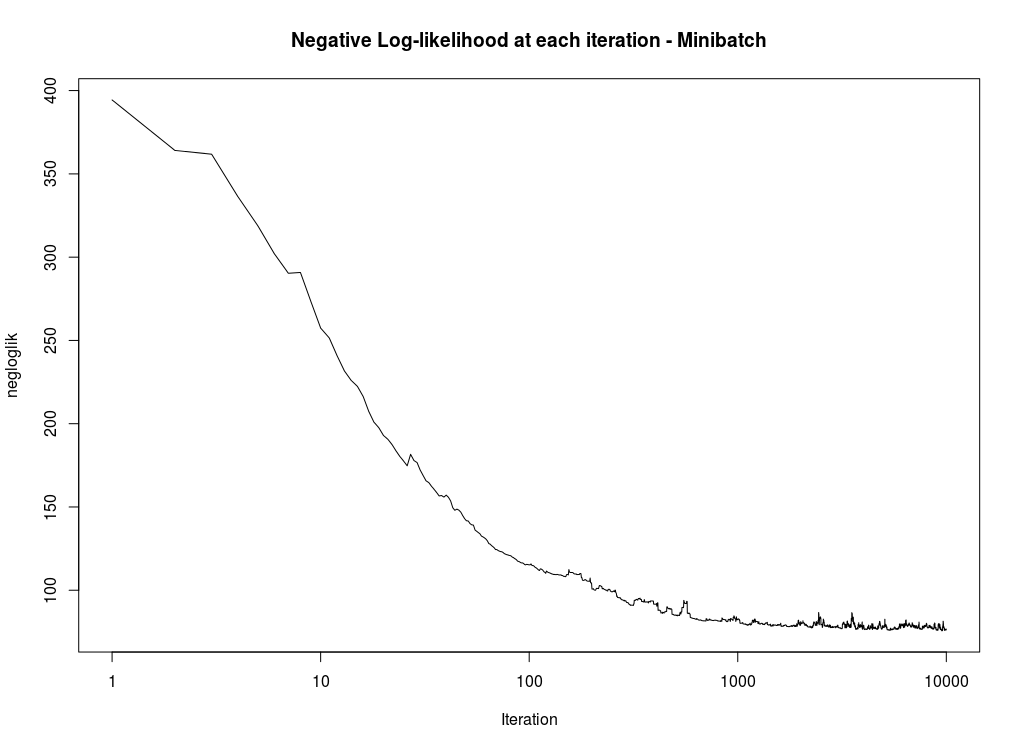
\includegraphics[width=\textwidth]{Rplot_minibatch01.png}

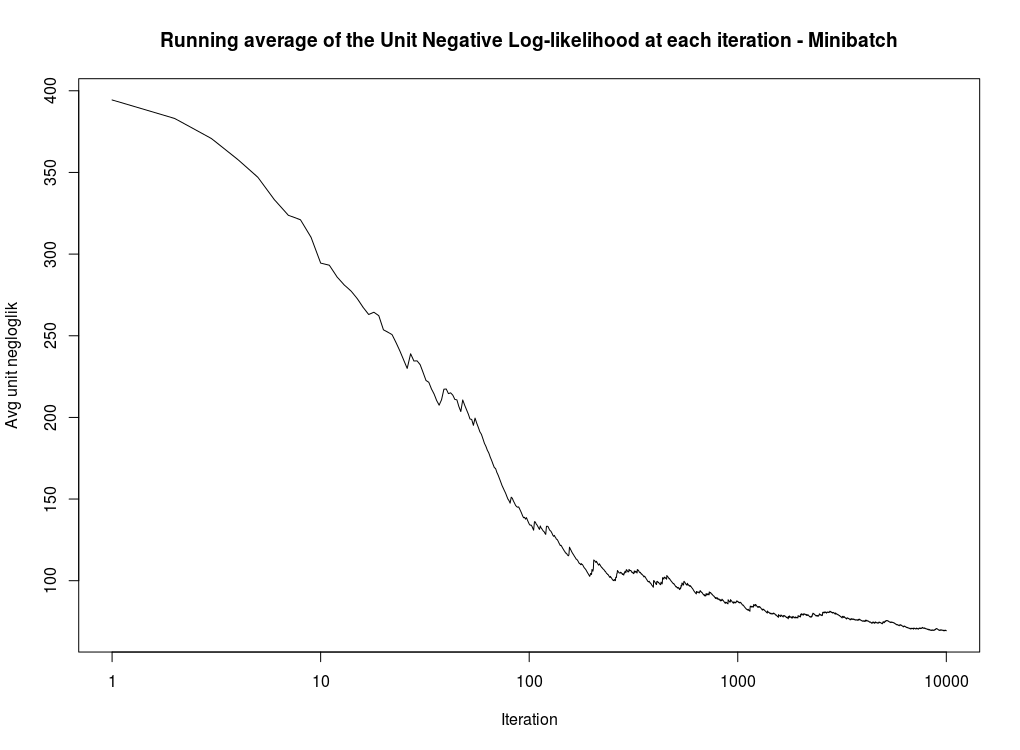
\includegraphics[width=\textwidth]{Rplot_minibatch02.png}

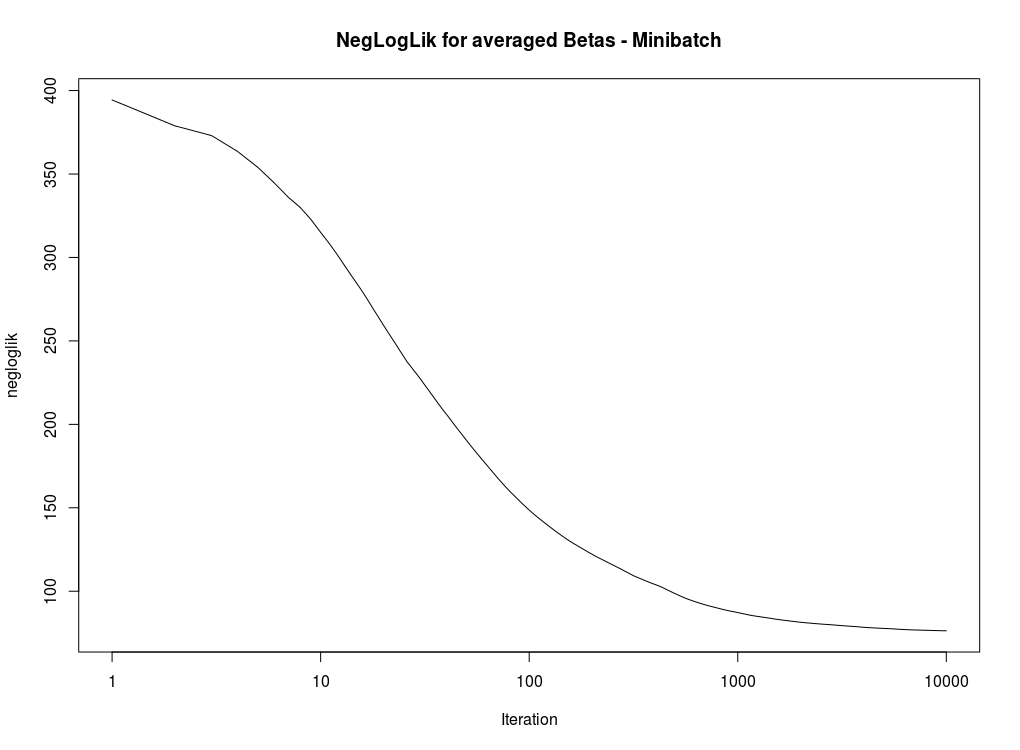
\includegraphics[width=\textwidth]{Rplot_minibatch03.png}

\subsubsection*{B)}

Again, running the code in appendix, we can observe how the AdaGrad algorithm fares.

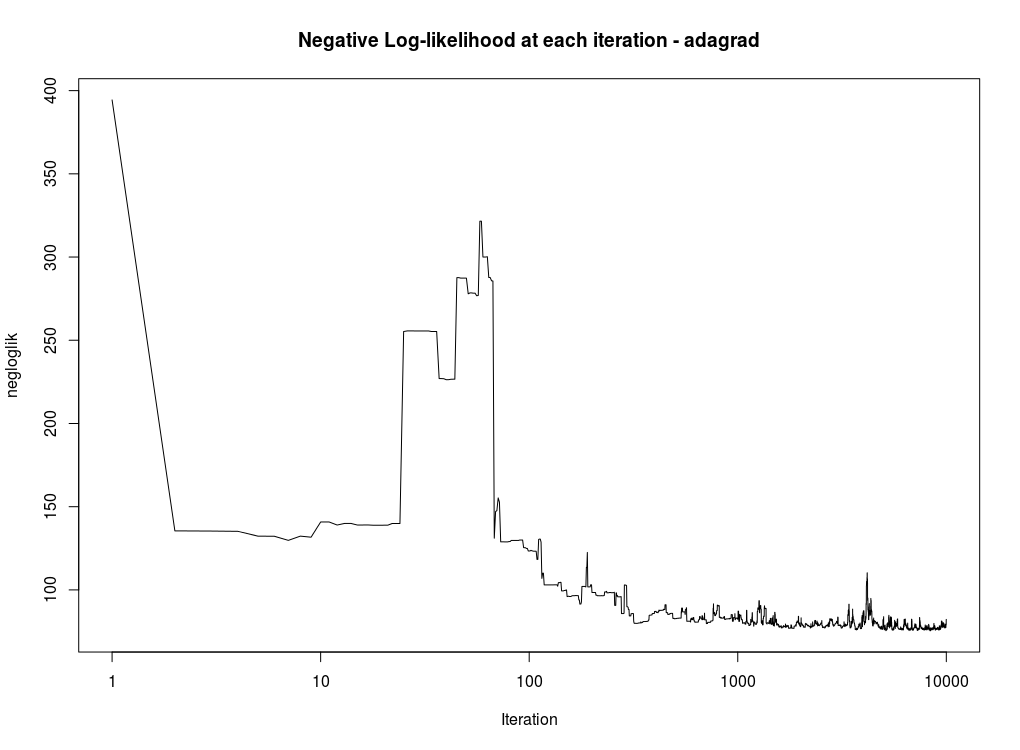
\includegraphics[width=\textwidth]{Rplot_AdaGrad01.png}

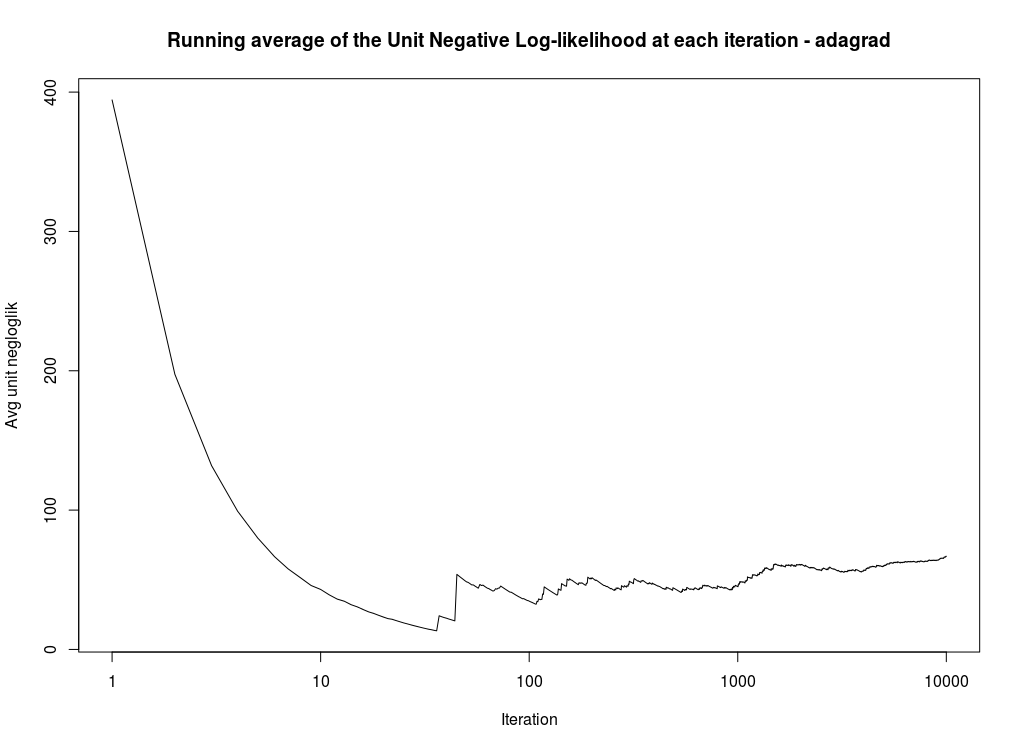
\includegraphics[width=\textwidth]{Rplot_AdaGrad02.png}

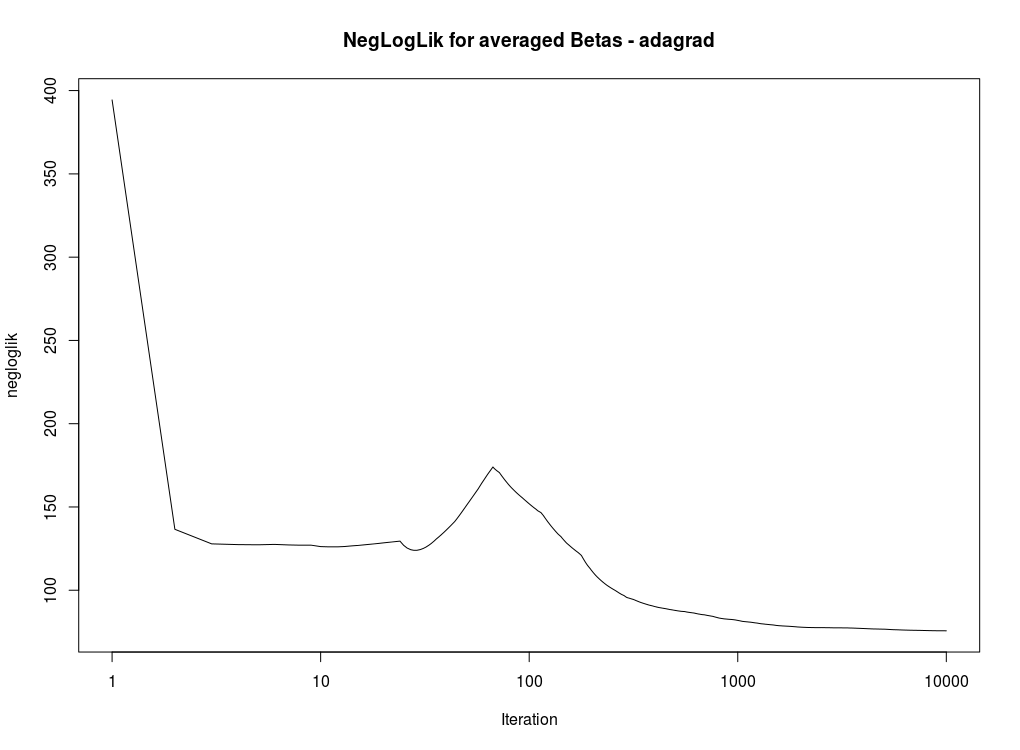
\includegraphics[width=\textwidth]{Rplot_AdaGrad03.png}

\subsubsection*{CODE)}

%[basicstyle=\tiny]
\begin{lstlisting}
library(Matrix)
library(microbenchmark)

negloglikelihood<-function(m,y,X,beta){
  total<-0
  N<-length(y)
  for(i in 1:N){
    Xtbeta<-crossprod(X[i,],beta)
    total<-total+(m[i]-y[i])*Xtbeta+m[i]*log(1+exp(-Xtbeta))} 
  return(total)}

gradient_negloglik<-function(m,y,X,beta){
  w<-1/(1+exp(-X%*%beta))
  S<-m*w-y
  grad<-t(X)%*%S
  return(grad)}

unit_negloglikelihood_v2<-function(unitM,unitY,unitX,beta){
  Xtbeta<-crossprod(unitX,beta)
  result<-(unitM-unitY)*Xtbeta+unitM*log(1+exp(-Xtbeta))
  return(result)}


unit_gradient_negloglik_v2<-function(unitM,unitY,unitX,beta){
  unitW<-1/(1+exp(-crossprod(unitX,beta)))
  S<-unitM*unitW-unitY
  grad<-unitX*S
  return(grad)}

line_search<-function(alpha,c1,rho,gradient,m,y,X,beta){
  while(negloglikelihood(m,y,X,(beta-alpha*gradient))>
        negloglikelihood(m,y,X,beta)-c1*alpha*crossprod(gradient)){
    alpha<-alpha*rho}
  return(alpha)}

minibatch_SGD<-function(m,y,X,beta0,alpha,c1,rho,maxstepnumber,sizebatch,sizewait){
  n<-dim(X)[1]
  unit<-sample(seq(1,n-sizebatch),1)
  endbatch<-unit+sizebatch
  gradient<-gradient_negloglik(m[unit:endbatch],y[unit:endbatch],
                               X[unit:endbatch,],beta0)/sizebatch
  stepsize<-line_search(alpha,c1,rho,gradient,m[unit:endbatch],
                        y[unit:endbatch],X[unit:endbatch,],beta0)
  betas<-matrix(NA,nrow=maxstepnumber,ncol=dim(X)[2])
  betas[1,]<-beta0
  negloglik<-numeric(maxstepnumber)
  negloglik[1]<-negloglikelihood(m,y,X,beta0)
  unit_negloglik<-numeric(maxstepnumber)
  unit_negloglik[1]<-negloglik[1]/n
  i<-1
  while(!(i==maxstepnumber)){
    i<-i+1
    beta1<-beta0-stepsize*gradient
    beta0<-beta1
    negloglik[i]<-negloglikelihood(m,y,X,beta0)
    unit_negloglik[i]<-unit_negloglikelihood_v2(m[unit],y[unit],X[unit,],beta0)
    betas[i,]<-beta0
    if(i%%sizewait==0){
      unit<-sample(seq(1,n-sizebatch),1)
      endbatch<-unit+sizebatch
      gradient<-gradient_negloglik(m[unit:endbatch],y[unit:endbatch],
                                   X[unit:endbatch,],beta0)/sizebatch
      stepsize<-line_search(stepsize,c1,rho,gradient,m[unit:endbatch],
                            y[unit:endbatch],X[unit:endbatch,],beta0)
    }else{
      unit<-sample(seq(1,n),1)
      gradient<-unit_gradient_negloglik_v2(m[unit],y[unit],X[unit,],beta0)}}
  return(list(betahat=beta0,negloglik=negloglik,
              unit_negloglik=unit_negloglik,betas=betas))}

data_wdbc<-read.csv("./wdbc.csv", header=FALSE)
X<-as.matrix(cbind(rep(1,569),scale(data_wdbc[,3:12])))
y<-data_wdbc[,2]
y<-as.numeric(y=="M")
m<-rep(1,569)

beta0<-rep(0,11)
alpha<-0.06
c1<-0.01
rho<-2/3
maxstepnumber<-10000
sizebatch<-10
sizewait<-47
res_minibatch_sgd<-minibatch_SGD(m,y,X,beta0,alpha,c1,rho,maxstepnumber,sizebatch,sizewait)

plot(res_minibatch_sgd$negloglik,
     main = "Negative Log-likelihood at each iteration - Minibatch",
     xlab="Iteration",ylab="negloglik",type="l",log="x")

running_avg_minibatch<-numeric(maxstepnumber)
running_avg_minibatch[1]<-res_minibatch_sgd$unit_negloglik[1]
for(i in 2:maxstepnumber){
  running_avg_minibatch[i]<-(running_avg_minibatch[i-1]*(i-1)+
							  res_minibatch_sgd$unit_negloglik[i])/(i)}
plot(569*running_avg_minibatch,
     main = "Running average of the Unit Negative Log-likelihood at each iteration - Minibatch",
     xlab="Iteration",ylab="Avg unit negloglik",type="l",log="x")

running_avg_beta_minibatch<-matrix(NA,nrow=maxstepnumber,ncol=11)
running_avg_beta_minibatch[1,]<-res_minibatch_sgd$betas[1,]
running_negloglik_minibatch<-numeric(maxstepnumber)
running_negloglik_minibatch[1]<-negloglikelihood(m,y,X,running_avg_beta_minibatch[1,])
for(i in 2:maxstepnumber){
  running_avg_beta_minibatch[i,]<-(running_avg_beta_minibatch[i-1,]*(i-1)+
  									res_minibatch_sgd$betas[i,])/(i)
  running_negloglik_minibatch[i]<-negloglikelihood(m,y,X,running_avg_beta_minibatch[i,])}
plot(running_negloglik_minibatch,
     main = "NegLogLik for averaged Betas - Minibatch",
     xlab="Iteration",ylab="negloglik",type="l",log="x")

AdaGrad_SGD<-function(m,y,X,beta0,stepsize,maxstepnumber,ada_eps){
  n<-dim(X)[1]
  p<-dim(X)[2]
  unit<-sample(seq(1,n),1)
  betas<-matrix(NA,nrow=maxstepnumber,ncol=p)
  betas[1,]<-beta0
  negloglik<-numeric(maxstepnumber)
  negloglik[1]<-negloglikelihood(m,y,X,beta0)
  unit_negloglik<-numeric(maxstepnumber)
  unit_negloglik[1]<-negloglik[1]/n
  gradient<-unit_gradient_negloglik_v2(m[unit],y[unit],X[unit,],beta0)
  diag_G<-gradient^2
  i<-1
  while(!(i==maxstepnumber)){
    i<-i+1
    beta1<-beta0-stepsize/sqrt(diag_G+ada_eps)*gradient
    beta0<-beta1
    negloglik[i]<-negloglikelihood(m,y,X,beta0)
    unit_negloglik[i]<-unit_negloglikelihood_v2(m[unit],y[unit],X[unit,],beta0)
    betas[i,]<-beta0
    unit<-sample(seq(1,n),1)
    gradient<-unit_gradient_negloglik_v2(m[unit],y[unit],X[unit,],beta0)
    diag_G<-diag_G+gradient^2}
  return(list(betahat=beta0,negloglik=negloglik,
              unit_negloglik=unit_negloglik,betas=betas))}

stepsize<-1
maxstepnumber<-10000
ada_eps<-0.0000001
res_adagrad_sgd<-AdaGrad_SGD(m,y,X,beta0,stepsize,maxstepnumber,ada_eps)

plot(res_adagrad_sgd$negloglik,
     main = "Negative Log-likelihood at each iteration - adagrad",
     xlab="Iteration",ylab="negloglik",type="l",log="x")

running_avg_adagrad<-numeric(maxstepnumber)
running_avg_adagrad[1]<-res_adagrad_sgd$unit_negloglik[1]
for(i in 2:maxstepnumber){
  running_avg_adagrad[i]<-(running_avg_adagrad[i-1]*(i-1)+
  							res_adagrad_sgd$unit_negloglik[i])/(i)}
plot(569*running_avg_adagrad,
     main = "Running average of the Unit Negative Log-likelihood at each iteration - adagrad",
     xlab="Iteration",ylab="Avg unit negloglik",type="l",log="x")

running_avg_beta_adagrad<-matrix(NA,nrow=maxstepnumber,ncol=11)
running_avg_beta_adagrad[1,]<-res_adagrad_sgd$betas[1,]
running_negloglik_adagrad<-numeric(maxstepnumber)
running_negloglik_adagrad[1]<-negloglikelihood(m,y,X,running_avg_beta_adagrad[1,])
for(i in 2:maxstepnumber){
  running_avg_beta_adagrad[i,]<-(running_avg_beta_adagrad[i-1,]*(i-1)+
  								  res_adagrad_sgd$betas[i,])/(i)
  running_negloglik_adagrad[i]<-negloglikelihood(m,y,X,running_avg_beta_adagrad[i,])}
plot(running_negloglik_adagrad,
     main = "NegLogLik for averaged Betas - adagrad",
     xlab="Iteration",ylab="negloglik",type="l",log="x")
\end{lstlisting}

\end{document}